 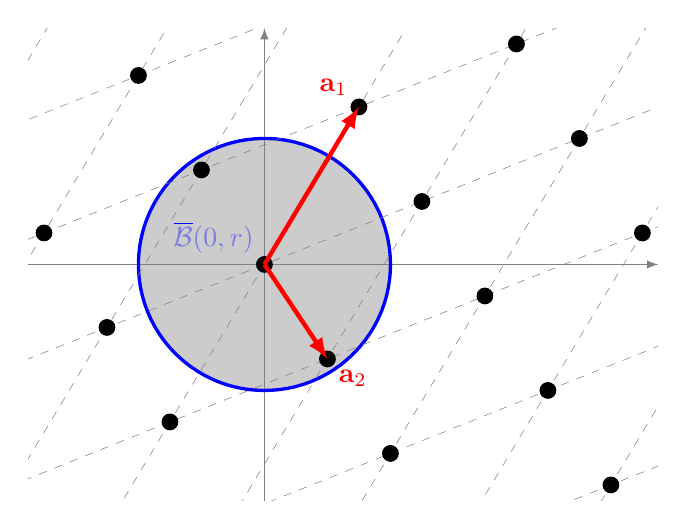
\begin{tikzpicture}
    \coordinate (Origin)   at (0,0);
    \coordinate (XAxisMin) at (-3,0);
    \coordinate (XAxisMax) at (5,0);
    \coordinate (YAxisMin) at (0,-3);
    \coordinate (YAxisMax) at (0,3);
    \draw [thin, gray,-latex] (XAxisMin) -- (XAxisMax);% Draw x axis
    \draw [thin, gray,-latex] (YAxisMin) -- (YAxisMax);% Draw y axis
    \draw[color=blue,very thick,fill=gray, fill opacity=0.4](0,0) circle(1.6) node [above left] {$\overline{\mathcal{B}}(0,r)$};

    \clip (-3,-3) rectangle (5cm,3cm); % Clips the picture...
    
    \pgftransformcm{1}{0.4}{0.6}{1}{\pgfpoint{0cm}{0cm}}
    \coordinate (Bone) at (0,2);
    \coordinate (Btwo) at (2,-2);
    \draw[style=help lines,dashed] (-14,-14) grid[step=2cm] (14,14);
    \foreach \x in {-7,-6,...,7}{% Two indices running over each
      \foreach \y in {-7,-6,...,7}{% node on the grid we have drawn 
        \node[draw,circle,inner sep=2pt,fill] at (2*\x,2*\y) {};
            % Places a dot at those points
      }
    }
    \draw [ultra thick,-latex,red] (Origin)
        -- (Bone) node [above left] {$\mathbf{a}_1$};
    \draw [ultra thick,-latex,red] (Origin)
        -- (Btwo) node [below right] {$\mathbf{a}_2$};
    
  \end{tikzpicture}